\chapter{Les projets}
La gestion des clients associe à chacun d'eux un ou plusieurs projets : il est donc nécessaire de visualiser la liste des projets pour chacun des clients. 
\begin{figure}[H]
	\centering
	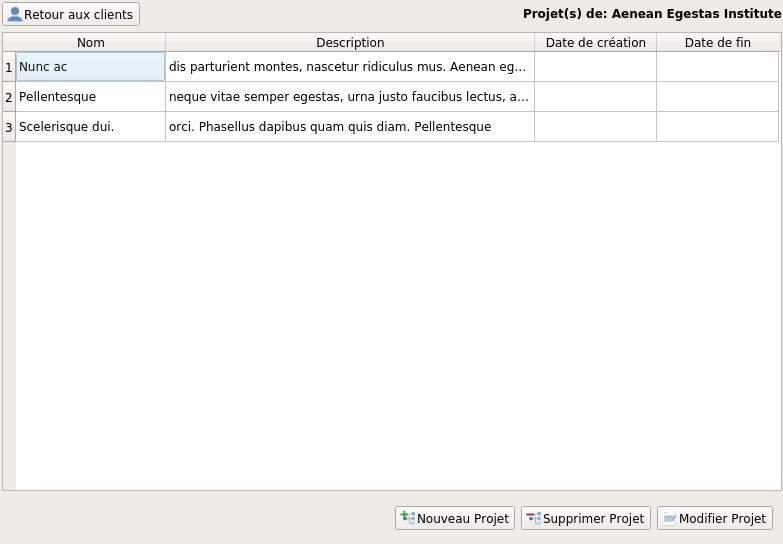
\includegraphics[width=12cm]{screens/projets.png}
	\caption{Gestion des projets d'un client}
\end{figure}

\section{Liste des projets\index{Projet!Liste}}
La liste des projets d'un client se trouve soit dans l'arborescence de la vue hiérarchique\index{Panneau!Hiérarchie} en déroulant la liste des projets d'un client soit en faisant un double clic sur l'un des clients de la liste du panneau centrale. Dans les deux cas, cela modifie le panneau principal qui contient maintenant la liste des projets pour le client comme le montre la figure ci-dessous.
\begin{figure}[H]
	\centering
	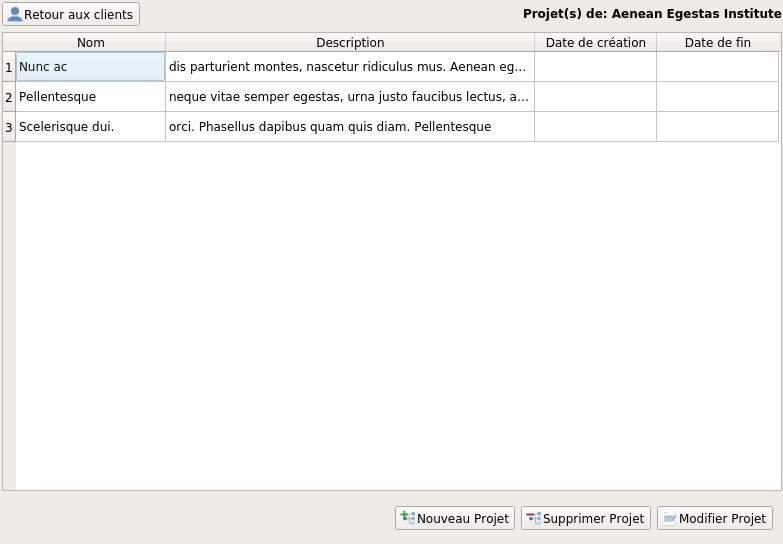
\includegraphics[width=10cm]{screens/projets.png}
	\caption{Liste des projets}
\end{figure}
La liste des projets contient les informations de chacun des projets c'est-à-dire un nom de projet, une description, les dates de début et de fin de projet. 

\section{Ajout d'un projet\index{Projet!Ajouter}}
L'ajout d’un projet peut se faire via le bouton <<Nouveau projet>> en bas du panneau principal.
Cependant, selon que le panneau central soit la liste des clients ou celle des projets, l'interface diffère. En effet, dans le premier cas il faut associer un projet à un client. 
C'est pour cela que la fenêtre propose un tableau avec la liste des clients afin de sélectionner celui auquel on veut associer un projet. 
Une barre de recherche permettant de retrouver facilement un client dans la liste est présente dans l'interface. Pour qu'un projet puisse être ajouté il devra obligatoirement être associé à un client et avoir un nom. 
Il est également possible d'ajouter une courte description et de mentionner le coût horaire ou journalier du projet. 
\begin{figure}[H]
	\centering
	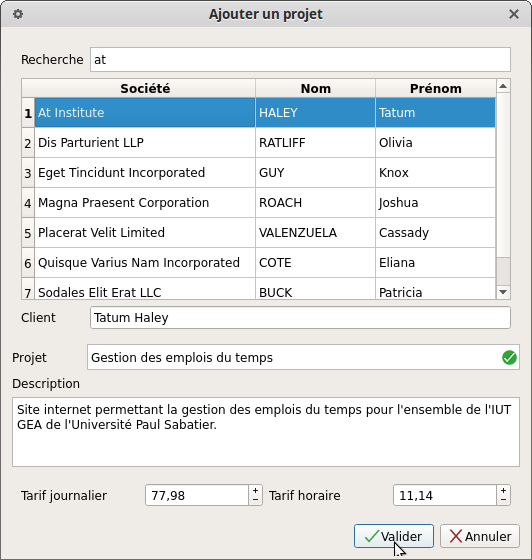
\includegraphics[width=7cm]{screens/ajouterProjet.png}
	\caption{Ajouter un projet}
\end{figure}
Dans le cas où le panneau central contient la liste des projets, cela signifie que ces projets sont ceux d'un client. C'est pourquoi, lorsqu'on clic sur le bouton <<Nouveau projet>>, celui-ci est automatiquement affecté au client courant. 
\begin{figure}[H]
	\centering
	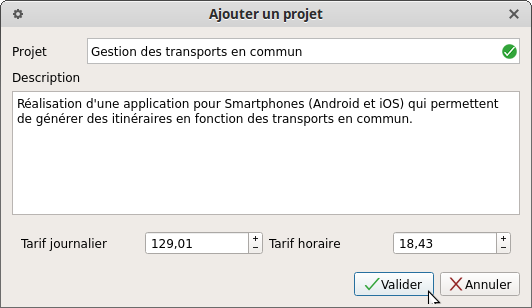
\includegraphics[width=7cm]{screens/ajouterProjetClient.png}
	\caption{Ajouter un nouveau projet à un client}
\end{figure}

\section{Édition d'un projet\index{Projet!Éditer}}
L’édition d’un projet a pour but de corriger d’éventuelles erreurs sur les informations d’un projet. Pour ce faire, il suffit de sélectionner un projet dans le tableau et de cliquer sur le bouton <<Modifier>> situé sous la liste des projets. 
La fenêtre est similaire à celle lors de l'ajout d'un projet à un client, seul diffère les champs qui sont pré-remplis. 
\begin{figure}[H]
	\centering
	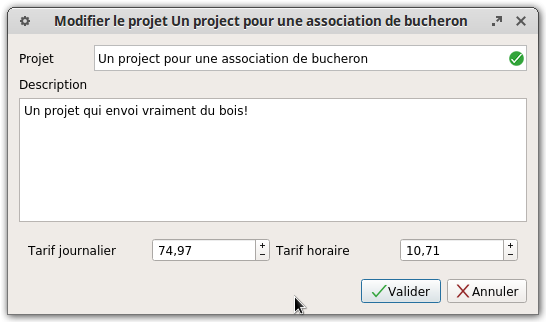
\includegraphics[width=7cm]{screens/editerProjet.png}
	\caption{Éditer un projet}
\end{figure}